\documentclass[11pt]{article}
\usepackage{tdt4310}
\usepackage[greek,english]{babel}
\usepackage{lmodern}
\usepackage[utf8]{inputenc}                     % Allow for non-ASCII input
\usepackage[T1]{fontenc}                         % Use rich fonts
\usepackage{times}
\usepackage{latexsym}
\usepackage{float}
\usepackage{amsmath}
\usepackage{booktabs} % For prettier tables
\usepackage{longtable} % If your table is too long for one
\usepackage{geometry} % Set page margins

\usepackage{svg}
\usepackage[toc,page]{appendix}

%%%%%%%%%%%%%%%%%%%%%%%%%%%%%%%%%%%%%%%%%%%%%%%%%%%%%
% Hyperlinks, you can choose different colours for different types of links; the defult colours are as below
\usepackage[colorlinks]{hyperref}
\hypersetup{
    linkcolor=black,	% internal cross-references; default red
    urlcolor=blue,	% default magenta
    citecolor=black,	% default green
   }
\urlstyle{same}	% if you want links in the same style as the rest of the text; default is typewriter style
\usepackage{doi}

%%%%%%%%%%%%%%%%%%%%%%%%%%%%%%%%%%%%%%%%%%%%%%%%%%%%%
% Graphics, tables and figures
\usepackage{graphicx}                           
\usepackage[table]{xcolor}
\usepackage{colortbl}
\usepackage{tcolorbox}
\usepackage{framed}
\usepackage{tabularx}
\usepackage{multicol}
\usepackage{multirow}
\usepackage{rotating}
\usepackage{array}
\usepackage{supertabular}
\usepackage{hhline}
\usepackage{subcaption}

% nicer table dividers
\usepackage{booktabs}
\usepackage{threeparttable}

% only needed if you want to pgfplots to draw figures
%\usepackage{tikzsymbols}
%\usepackage{pgfplots}

%%%%%%%%%%%%%%%%%%%%%%%%%%%%%%%%%%%%%%%%%%%%%%%%%%%%%
% comments and notes, useful while working on a draft - change the option 'draft' to 'disable' in the final version
\usepackage[draft]{todonotes}
\usepackage{verbatim}     % allow for longer comments

%%%%%%%%%%%%%%%%%%%%%%%%%%%%%%%%%%%%%%%%%%%%%%%%%%%%%
% BIBLIOGRAPHY STUFF

\usepackage[round]{natbib}

%%%%%%%%%%%%%%%%%%%%%%%
% uncomment if instead using biber as backend
\begin{comment}
\usepackage[backend=biber,
            bibstyle=apa,
            citestyle=authoryear,
            natbib=true,
            url=false,
            doi=false,
            hyperref=true,
            apamaxprtauth=99,
            maxcitenames=2,
            language=british,
            uniquelist=false,
            ]{biblatex}         % Correct citations

% Bibliography (+ hacks)
\addbibresource{bib/references.bib}
\addbibresource{bib/bibliography.bib}
\DeclareLanguageMapping{british}{british-apa}
\setlength\bibitemsep{2\itemsep}
\patchcmd{\bibsetup}{\interlinepenalty=5000}{\interlinepenalty=10000}{}{}
\let\citep\parencite
\let\cite\textcite
% Make the whole cite a hyperref
\DeclareCiteCommand{\textcite}
{\boolfalse{cbx:parens}}
{\usebibmacro{citeindex}%
    \printtext[bibhyperref]{\usebibmacro{textcite}}}
{\ifbool{cbx:parens}
    {\bibcloseparen\global\boolfalse{cbx:parens}}
    {}%
    \multicitedelim}
{\usebibmacro{textcite:postnote}}
\DeclareCiteCommand{\parencite}[\mkbibparens]
{\usebibmacro{prenote}}
{\usebibmacro{citeindex}%
    \printtext[bibhyperref]{\usebibmacro{cite}}}
{\multicitedelim}
{\usebibmacro{postnote}}
\end{comment}
% end biber part
%%%%%%%%%%%%%%%%%%%%%%%

%%%%%%%%%%%%%%%%%%%%%%%%%%%%%%%%%%%%%%%%%%%%%%%%%%%%%
% HYPHENATION DEFINITIONS

\usepackage{hyphenat}

% add correct hyphenations as needed
\hyphenation{hash-tag Sem-Eval}
\hyphenation{cyber-bully cyber-bullying}
%%%%%%%%%%%%%%%%%%%%%%%%%%%%%%%%%%%%%%%%%%%%%%%%%%%%%

\title{Comparative Analysis of Generative and Neural Topic Modeling Techniques Applied to Modern Greek Political Corpora}

\author{
  Nikolaos Giannakopoulos \and Dionysios Rigatos\\
  Norwegian University of Science and Technology \\
  Athens University of Economics and Business \\
  {\tt \{nikolagi, dionysir\}@stud.ntnu.no}}

\date{Report in TDT4310, NTNU, \today}
\begin{document}
\maketitle
\begin{abstract}
In this project, we explore a variety of topic modeling techniques with a focus on their application to a corpus of modern Greek political texts. We analyze and compare several classic generative models with state-of-the-art neural models, which provides an extensively modular framework for deep learning based topic modeling. By leveraging these sophisticated models, we aim to address the challenges of unsupervised topic modeling, such as their interpretability and incompatibility with quantitative metrics. Our approach involves a sophisticated experimental setup where models are fine-tuned and compared using a variety of topic coherence, diversity and similarity metrics. This study not only tests the effectiveness of different topic modeling techniques but also examines their application in a linguistically diverse dataset and the challenges that come with it - such as text pre-processing - providing insights that could benefit further research in the area of topic modeling for Greek corpora.
\end{abstract}

\section{Introduction}
\label{sec:Introduction}
In such a rapidly expanding field like text analytics and natural language processing and with the power of deep neural models, tackling multilingual tasks is more accessible than ever. The integration of such technologies is rapidly transforming the landscape, opening up a great amount of possibilities for both advancing multilingual research as well as creating useful models with specific applications in these languages. In our case, we leverage an array of topic models using the Optimizing and Comparing Topic Models Is Simple (OCTIS) \citep{Terragni;Fersini;Galuzzi;Tropeano;Candelieri;21} library and BERTopic \citep{grootendorst2022bertopic} so as to perform an analysis on a corpus of modern Greek political speeches and statements issued by the Prime Minister's office from 2012 to 2024. Our frozen-in-time model approach will make full use of the unlabeled data and allowing these models to achieve optimal performance in extracting topics for offline, unsupervised tasks aimed primarily at dataset evaluation.

This project not only presents an analytical study but also sets the foundational framework by outlining the dataset selection process, addressing the unique challenges of pre-processing texts in the Greek language, and understanding the rationale behind our methodological choices. With our approach, we aim to contribute to both the academic and practical stakeholders in the field of modern Greek text analysis.
\section{Theoretical Background}
\label{sec:background}
\subsection{Topic Modeling}
Topic modeling is a statistical modeling technique utilized in the fields of natural language processing and text mining among others so as to identify and extract the topics or themes present within a large collection of documents. It operates on the premise of the distributional hypothesis as explained by \cite{Harris:54} - documents encompass a mixture of various topics that consist of frequently co-occurring words. 

Implementations of such models are usually trained using unsupervised learning methods, thus allowing them to uncover more than what is known about a document by providing insights into large and unstructured text datasets by discovering the latent structures within them. 

\subsection{Topic Diversity}
\label{sec:topicDiversity}
The Topic Diversity score measures the lexical diversity across topics in a corpora by examining the ratio of unique top-K words across all of the topics to the total number of top-K words.
\begin{align*}
TD = \frac{|\text{Unique\_TopK\_Words}|}{K \times |\text{Τopics}|}
\end{align*}

\subsection{Topic Coherence Metrics}
\label{sec:topicCoherence}
Topic Coherence is a quantitative assessment of how well topics can be explained by the corpora they were generated from. 
\subsubsection{UMass Coherence}
The UMass coherence score (\cite{Mimno;Wallach;Talley;Leenders;McCallum:11}) assesses topic quality by measuring how words that belong to a coherent topic are more likely to appear together in the same documents more frequently than words that do not belong to a coherent topic. As such, coherent topics will have word pairs that show a higher degree of co-occurrence and higher $C(t)$ values. It is formulated as such:

\begin{align*}
C(t; V(t)) = \sum_{m=2}^{M} \sum_{l=1}^{m-1} \log \left( \frac{D(v_{t,m}, v_{t,l}) + 1}{D(v_{t,l})} \right)
\end{align*}
\subsubsection{CV Coherence}
\label{sec:CVCoherence}
The CV coherence score (\cite{Roder;Both;Hinneburg:15}) measures the semantic similarity between high-scoring words in topics, considering a wide window of words instead of just adjacent words. This score uses Normalized Pointwise Mutual Information (NPMI) (\cite{Aletras;Stevenson:13}) and the cosine similarity between word vectors of the top-ranked words within the topics.

\subsection{Topic Similarity Metrics} 
\label{sec:topicSimilarity}
Topic similarity is a quantitative assessment of how similar topics are to each other.

\subsubsection{Pairwise Jaccard Similarity}
The Pairwise Jaccard Similarity score, in the context of topic modeling, measures the similarity between different topics by comparing the sets of documents associated with each topic. The Jaccard Similarity Index (\cite{Jaccard:40}), calculated for two sets, is the ratio of the number of elements in the intersection of the sets to the number of elements in their union. Applied to topic modeling, if each topic is represented as a set of documents that prominently feature the topic, the Jaccard Index can quantify how similar two topics are based on their document overlap. A higher Jaccard score indicates a greater overlap and thus higher similarity between the topics.

\subsection{Word Embeddings}
Word embeddings \citep{mikolov2013efficient} are a class of techniques where words are represented by vectors of real numbers in a low-dimensional space. These vectors try to capture the semantic meaning of words and are constructed in such a way that semantically similar words are closer together in that vector space. Techniques like Continuous Bag-of-Words (CBOW) and skip-gram are used to learn these embeddings from large text corpora.

\subsection{Clustering}
Clustering refers to unsupervised machine learning techniques that group data points into clusters based on distance (e.g. Euclidean distance), or similarity (e.g. cosine similarity) measures. The goal is to organize data in such a way that those who share similar attributes are put in the same cluster.

\subsection{Dimensionality Reduction}
As dimensions increase we face something often referred to as the curse of dimensionality \citep{Bellman:57}. Traditional distance measures don't work and finding meaningful clusters becomes challenging. Dimensionality reduction refers to a set of techniques aimed at transforming data from a high-dimensional space to a lower one, while preserving the important characteristics of the data, so we can apply traditional distance measuring and clustering techniques. 

\subsection{Word Weighting / TF-IDF}
Word weighting refers to techniques used for calculating the importance of words within a set of texts (corpus). 

The most popular amongst these techniques is Term Frequency - Inverse Document Frequency (TF-IDF) \citep{SALTON1988513}. Term Frequency $tf_{t,d}$ is a measure for how often a word appears in single document, while document frequency counts how rare a word is within a corpus by measuring the amount of documents that contain that word.

\begin{equation}\label{tf-idf}
W_{t,d} = tf_{t,d} \cdot \log(\frac{N}{df_t})
\end{equation}

\subsection{Transformer Architecture}
Transformers \citep{vaswani2023attention} are a deep learning architecture relying on the concept of Attention \citep{bahdanau2016neural}. Self-attention allows the model to focus on different parts of the input sequence, by assigning different weights to different input tokens. These weights, in contrast to other types of Neural Networks, are not learned during training, but are computed based on the input sequence and can change for each input token. This allows the model to learn dependencies between tokens that are far apart in the input sequence, which is a key advantage of transformers compared to other architectures. 

% \newcommand\emc{-~~~~}
% \begin{table}[t!]
% \centering
% \caption{Example table (F$_1$-scores)}
% \begin{tabular}{c|c|rrrrrr}
% \toprule
% Langs                       & Source                 & \multicolumn{1}{c}{Lang1} & \multicolumn{1}{c}{Lang2} & \multicolumn{1}{c}{Univ}                                                     & \multicolumn{1}{c}{NE}    & \multicolumn{1}{c}{Mixed} & \multicolumn{1}{c}{Undef} 
% \\ \midrule
% \multirow{5}{*}{EN-HI} & FB+TW                  & 54.22 & 22.00 & 19.70 & 4.00  & 0.05  & 0.03  \\
%                        & FB                     & 75.61 & 4.17  & 18.00 & 2.19  & 0.02  & 0.01  \\  
%                        & TW                     & 22.24 & 48.48 & 22.42 & 6.71  & 0.08  & 0.07  \\  
%                        & Vyas                   & 54.67 & 45.27 & 0.06  & \emc  & \emc  & \emc  \\ 
%                        & FIRE                   & 45.57 & 39.87 & 14.52 & \emc  & 0.04  & \emc  \\ \midrule
% \multirow{2}{*}{EN-BN} & TW                     & 55.00 & 23.60 & 19.04 & 2.36  & \emc  & \emc  \\ 
%                         &  FIRE                 & 32.47 & 67.53 & \emc  & \emc  & \emc  & \emc  \\ \midrule
% EN-GU                  & FIRE                   & 5.01  & {\bf 94.99} & \emc  & \emc  & \emc  & \emc  \\ 
% \midrule
% DU-TR                  & Nguyen                 & 41.50 & 36.98 & 21.52 & \emc  & \emc  & \emc  \\ \midrule

% EN-ES                  & \multirow{4}{*}{\rotatebox[origin=c]{90}{EMNLP}} 
%                                                 & 54.79 & 23.50 & 19.35                                                    & 2.08  & 0.04  & 0.24  \\ 
% EN-ZH                  &                        & 69.50 & 13.95 & 5.88                                                     & 10.60 & 0.07  & \emc     \\ 
% EN-NE                  &                        & 31.14 & 41.56 & 24.41                                                    & 2.73  & 0.08  & 0.08  \\ 
% AR-AR                  &                        & 66.32 & 13.65 & 7.29                                                     & 11.83 & 0.01  & 0.90    \\ \bottomrule
% \end{tabular}
% \label{tab:ExampleTable}
% \end{table}

\section{Related Work}
\label{sec:related_work}
As it was previously mentioned, machine learning has become more versatile than ever when it comes to applications in under-represented languages. Topic Modeling heavily benefits from this versatility as it has applications in both supervised and unsupervised tasks - providing a relevant solution to the extraction of information from large corpora. 

As shown by \cite{Panagiotis;22}, state-of-the-art (SOTA) solutions such as BERTopic can lead to impressive results in language-specific tasks - something confirmed thanks to the availability of labels in their experiments. Their approach yielded acceptable quantitative metrics in both topic quality and classification of labeled corpora, while the qualitative aspect was also satisfactory. 

Our approach will rely heavily on manually gathered data from a specific domain (political publications) and in a strictly unsupervised context. On top of that, we aim to show that a thorough exploration of preprocessing techniques can significantly boost the performance of classic topic modeling algorithms. Additionally, we look for the optimal language-specific tools to help us achieve that which - in a way - evaluates them in a practical scenario. Finally, we will experiment generously with different modular components and hyperparameters in BERTopic, as well as with topic representation models for improved clarity in the outputs. Tackling this task with the big image in mind is very likely to yield interesting results at every single step of the analysis.
\section{Architecture \& Approach}
% OR: \section{Model}
\label{sec:architecture}
\subsection{Exploratory Data Analysis}
In this section we will go over the dataset chosen for this task, the preprocessing pipeline implemented as well as the a-priori insights we can extract regarding its contents.

\subsubsection{Dataset}
The dataset used in this analysis consists of speeches and statements gathered from the official website of the Office of the Greek Prime Minister in the time period between 2012 and 2024. It was fetched and assembled by a custom-built web page scraper, yielding approximately $2030$ distinct publications. 

The dataset is primarily in Greek, with a minority of English or French phrases/words. These publications are official transcripts and/or summaries of speeches and statements given by the active prime minister at the period. No other filtering was applied in the initial construction of the dataset other than the aforementioned time frame. While the speeches and the statements were loaded independently, a merged version of the data will be used in all of the tasks presented as they have an identical format, as shown in Table \ref{tab:dataset}.

\begin{table}[H]
\centering
\begin{tabular}{c|c|l}
\toprule
\textbf{Field} & \textbf{Type} & \multicolumn{1}{c}{\textbf{Description}} \\
\midrule
date   & str & Publication Date \\
id     & int & Publication ID \\
url    & str & Publication URL \\
title  & str & Publication Title \\
text   & str & Publication Content \\
\bottomrule
\end{tabular}
\caption{Dataset Attributes}
\label{tab:dataset}
\end{table}

\subsubsection{Data Preprocessing}
Our dataset consists of long texts in Greek, with a lot of repetitive language and - due to its context - legalese. OCTIS provides classes for easily preprocessing and storing the dataset, which may then be used as input in any of its algorithms for training and evaluation. One drawback of OCTIS' provided preprocessing is that it is black-box - it uses spaCy \citep{spacy:17} to modify the data and construct the expected dataset class. While spaCy provides support for processing Greek corpora, its lemmatization pipeline was unable to reduce most of the words to their root forms sufficiently. This was especially apparent in less mainstream words, which are quite common in official speeches and statements, as well as verbs. 

In order to overcome this issue we built a custom and OCTIS-compatible preprocessor based on Stanford's Stanza (\cite{Stanza:20}). Stanza supports the usage of external, custom-made models for the processing steps. While Greek is natively supported, we opted for a more specialized approach on lemmatization for the Greek language. As presented by \cite{Prokopidis;Piperidis:20} in A Neural NLP toolkit for Greek - their hybrid lexicon and part-of-speech based lemmatizer will be used so as to achieve more accurate conversions to root forms and therefore avoid the repetition of lexical cognates when generating topics. The difference between the two pipelines was not trivial and almost eliminated the issue of monolectic topics. With our pipeline prepared, there is a series of additional steps to be performed so as to build our training-ready dataset. 


Stopword removal will be applied using the union of spaCy's Greek el\_core\_news\_sm and English en\_core\_news\_sm. In fact, stopwords will be lemmatized and will be removed from the post-lemmatized text for higher coverage as Greek is quite a versatile language and these lists were not exhaustive. Removal of numbers and punctuation marks was also applied so as to have a more relevant vocabulary and ensure that words are not entangled between punctuation marks.

Word weighting with TF-IDF was used in order to maximize the relevance of the words present in our vocabulary in order to assist with the generation of topics. Specifically, all words present in more than $20\%$ or less than $1\%$ of the texts were omitted from the vocabulary. Additionally, a text had to consist of at least 20 words in order to be counted in as a data point. Finally, the minimum word length was set to 4, immediately excluding a plethora of context-lacking phrases. 

While the OCTIS models require preprocessing in order to produce acceptable result, unlike BERTopic which according to its documentation performs better when the input data is unprocessed and performs data processing later in its pipeline.

\subsubsection{Understanding The Data}
Instead of tackling the task blind, it is generally a good idea to extract some statistics prior to the analysis. This helps in spotting possible biases, imbalances or errors in the dataset.

\begin{figure}[H]
\centering
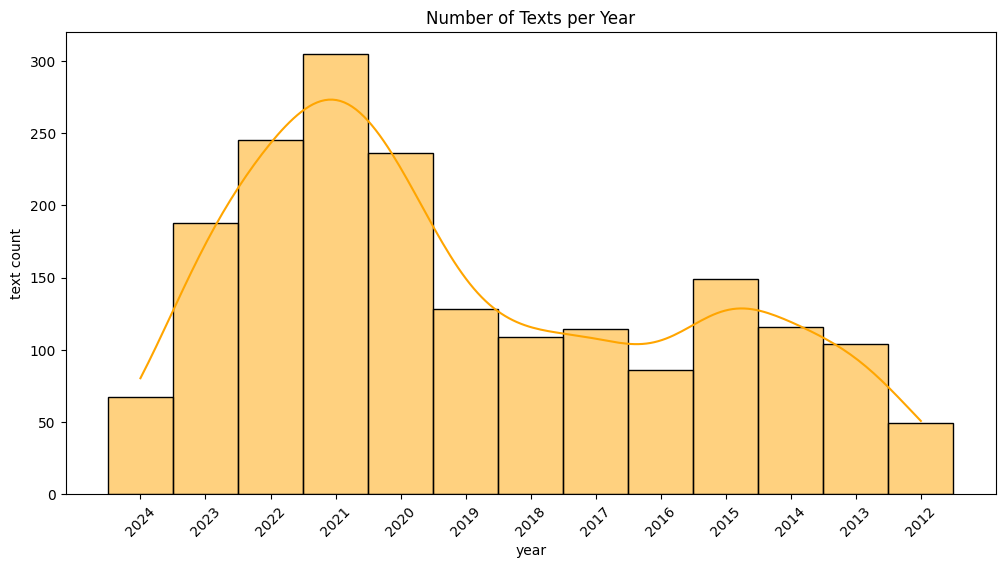
\includegraphics[width=0.8\columnwidth]{figs/eda_texts.png}
\caption[]{Count of data samples per year}
\label{fig:EDA_texts}
\end{figure}

As seen in Figure \ref{fig:EDA_texts}, our data is imbalanced in the sense that there has been a lot of publication activity from the Office of the Greek Prime Minister in the post-COVID era, meaning we might see an increased amount of recent topics compared to the mid-2010's. 

\begin{table}[H]
\centering
\caption{Selected Common Words by Year}
\label{tab:commonwords}
\begin{tabular}{@{}p{1cm}p{5cm}p{4cm}@{}} % Adjust the column width and alignment if necessary
\toprule
\textbf{Year} & \textbf{Common Words} & \textbf{Topic Description} \\
\midrule
2022 & \textgreek{ενεργειακός, ψηφιακός, τουρισμός, πηγή, πόλεμος} & Energy, Digital, Tourism, War \\
2021 & \textgreek{εμβολιασμός, ψηφιακός, εμβολιάζω, υφυπουργός, γραμματέας} & Vaccines, Digital Campaigns \\
2018 & \textgreek{μνημόνιο, περιφέρεια, παραγωγικός, νησί} & Memorandum, County, Island \\
2013 & \textgreek{πλεόνασμα, κόμμα, ανταγωνιστικότητα, ανεργία} & Surplus, Competitiveness, Unemployment \\
\bottomrule
\end{tabular}
\begin{tablenotes}
  \small
  \item \textit{Complete table available at Appendix \ref{sec:appA} Table \ref{appA:words_per_year}}
\end{tablenotes}
\end{table}



As we see in Table \ref{tab:commonwords}, we can also take a quick look at the most common words that appear in our texts, per year, as a taste of what to expect when generating topics.

\subsection{OCTIS Models}

Optimizing and Comparing Topic Models Is Simple (OCTIS) (\cite{Terragni;Fersini;Galuzzi;Tropeano;Candelieri;21}) is a library that encapsulates the preprocessing, optimization, training, evaluation and comparison of topic models. It contains a plethora of topic model algorithm implementations and metrics and thus will be used throughout so as to provide a platform for our chosen methods in this analysis. In this sub-section we will briefly go over the OCTIS-provided algorithms we will use in our experiments.

\subsubsection{Latent Semantic Indexing} 
Latent Semantic Indexing (also known as Latent Semantic Analysis, \cite{Landauer;Thomas;Foltz;Peter;Laham;Darrell:98}) is one of the first approaches in topic modeling that attempts to overcome the issue of variability in language when trying to retrieve relevant topics. It is able to extract context and capture semantic similarities between different words.

The algorithm initially constructs a weighted document-term matrix which stores the importance of each word based both on term frequency and inverse document frequency (tf-idf). This high-dimensional sparse matrix is then decomposed into three intermediate matrices using Singular Value Decomposition (SVD). These matrices are the term-concept vector matrix $W$, the singular value matrix $S$ and the concept-document vector matrix $P$. By picking the most significant singular values (columns) from $S$, the original matrix is essentially truncated and thus its dimensionality is reduced while keeping the maximum possible context. 

\subsubsection{Latent Dirichlet Allocation}
Latent Dirichlet Allocation (LDA) (\cite{Blei;Ng;Jordan:03}) is a generative probabilistic model designed for the analysis and decomposition of collections of discrete data sets into a predetermined number of topics. It is predicated on the construction of a Bayesian model where documents are conceptualized as random mixtures over latent topics and each topic is characterized by a specific distribution over words. Documents are generated by sampling words from these topic-specific distributions.

It fundamentally operates using a fixed K-dimension Dirichlet distribution. As seen in Figure \ref{fig:LDA_Plate}, the parameters include $\alpha$ and $\beta$, which are hyperparameters that set the prior distributions over document-topic mixtures and topic-word mixtures respectively. Additionally, $\theta$ represents the distribution of topics in a specific document. Finally, $z$ assigns topics to individual words and $w$ denotes the distribution of words for each topic, capturing the semantic essence. This assignment over the $N$ words is repeated for all the documents $D$.

\begin{figure}[H]
\centering
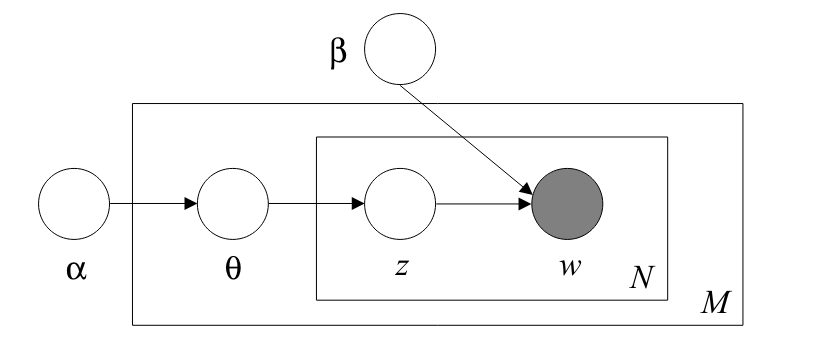
\includegraphics[width=0.5\columnwidth]{figs/lda_plate.png}
\caption[Latent Dirichlet Allocation Plate]{Plate representation of LDA
(adapted from \cite{Blei;Ng;Jordan:03})}
\label{fig:LDA_Plate}
\end{figure}

\subsubsection{Hierarchical Dirichlet Process} 
%https://www.cs.cmu.edu/~epxing/Class/10708-14/scribe_notes/scribe_note_lecture20.pdf
%https://mlg.eng.cam.ac.uk/zoubin/tut06/ywt.pdf
%https://people.eecs.berkeley.edu/~jordan/papers/hdp.pdf
%https://www.gatsby.ucl.ac.uk/~ywteh/research/npbayes/dp.pdf

Hierarchical Dirichlet Process (HDP) \citep{Teh;Jordan;Beal;Blei:06} is a topic modeling technique that extends the capabilities of LDA by allowing for an infinite number of topics across documents. While LDA requires pre-specifying dimensionality of the Dirichlet distribution (number of topics), HDP overcomes this limitation by leveraging the Dirichlet Process (DP) to model a potentially infinite number of topics, thereby providing a more flexible modeling approach. DP is an extra level added to the model.

\subsubsection{Product of Experts Latent Dirichlet Allocation}
%https://arxiv.org/pdf/1703.01488.pdf

Product of Experts Latent Dirichlet Allocation (ProdLDA) \citep{Srivastava;Sutton:17}, is a topic model that enhances the conventional LDA by modifying its underlying generative process. Unlike LDA, which represents documents as mixtures of topics where each word's generation is attributed to a single topic, ProdLDA redefines this structure by modeling the generation of words in a document as a Product of Experts \citep{hinton1999products}.

This simple yet important distinction allows ProdLDA to overcome a limitation of LDA where its generative process tends to yield less specific, and at times, less interpretable topics because the likelihood of word generation is averaged over the topics. 


\subsubsection{Honorable Mentions}
% %(https://papers.nips.cc/paper_files/paper/2000/hash/f9d1152547c0bde01830b7e8bd60024c-Abstract.html)

Non-negative Matrix Factorization (NMF) is a machine learning algorithm aimed at reducing the dimensionality of non-negative data by breaking it down into two matrices revealing underlying patterns, similar to LSI. While not natively a topic model, it is popular thanks to its ability to reduce dimensionality and produce coherent topics.

\subsection{BERTopic}
\label{sec:bertopic}

The previously mentioned algorithms rely on bag-of-word representations, which ignore the semantic relationships between words. Word embeddings and the emergence of Transformer-based models, such as Bidirectional Encoder Representations from Transformers (BERT) \citep{devlin2019bert} allow texts to be represented in such a way that similar texts are put together in the vector space. Then, as proposed by \citeauthor{sia-etal-2020-tired} \citeyearpar{sia-etal-2020-tired}, those embeddings can be clustered with each cluster representing a different topic.

BERTopic \citep{grootendorst2022bertopic} builds on this and combines clustering with a novelty class-based TF-IDF (c-TF-IDF) to create coherent topics from the created clusters. 

The steps of a BERTopic process, as seen in Figure \ref{fig:bertopic_architecture}, include creating embeddings of the documents, reducing the dimensions of those embeddings and then performing clustering. After that c-TF-IDF weighs the words present in each cluster to create topic representations.

\begin{figure}[H]
\centering
\includesvg{figs/bertopic.svg}
\caption[https://maartengr.github.io/BERTopic/algorithm/algorithm.html]{BERTopic Architecture (figure from Grootendorst Maarten)\footnotemark}}
\label{fig:bertopic_architecture}
\end{figure}
\footnotetext{https://maartengr.github.io/BERTopic/algorithm/algorithm.html}

BERTopic's other advantage lies in its modularity where each step algorithm of each step can be replaced with a different one.

\subsubsection{Sentence Transformers}
Similar to how traditional word embedding techniques create numerical vectors to make word representations, sentence transformers, as the name suggests, are able to generate embeddings for a large collections of tokens, creating vector representations for whole documents, sentences or paragraphs.

BERTopic for this step uses the Sentence-BERT (SBERT) framework \citep{reimers2019sentencebert} which consists of pre-trained Transformer-based language models. The SBERT framework provides many pre-trained models but any model can be used for creating text representations, such as models provided by Spacy, Gensim and Scikit-Learn Embeddings,

\subsubsection{Uniform Manifold Approximation and Projection for Dimension Reduction (UMAP)}
Sentence embeddings created by SBERT exist in a high dimensional space and, as found by \citeauthor{steinbachChallengesClusteringHigh2004} and \citeauthor{10.1007/3-540-49257-7_15}, traditional clustering techniques don't work well in high dimensions. The solution to that is reducing the dimensions. 

Techniques such as Principal Component Analysis (PCA) and t-Distributed Stochastic Neighbor Embedding (t-SNE) are widely used dimensionality reduction but BERTopic uses UMAP \citep{mcinnes2020umap}, which has shown to better preserve local features when reducing to as low as 2 dimensions.
\subsubsection{HDBSCAN}
After the document embeddings have reduced in dimensions, the clustering is performed with a hierarchical variation of Density-Based Spatial Clustering of Applications with Noise (DBSCAN).


DBSCAN \citep{10.5555/3001460.3001507} is a clustering algorithm that identifies dense regions of points that exist within a certain distance from each other and adding them to the same cluster. More specifically, it works with two parameters: \textgreek{ε}, which specifies the radius of the circle around each data point and minimum points, which specifies the least amount of points needed to form a cluster. Points with enough neighbors are core points of a cluster, whereas points far from any neighborhood are classified as noise.

Hierarchical DBSCAN (HDBSCAN) \citep{McInnes2017} performs DBSCAN with varying epsilon values, trying to find the one that gives the best stability. In this way, clusters of varying densities are created.

\subsubsection{c-TF-IDF}
Each cluster created by HDBSCAN represents a single topic. Depending on our corpus, each cluster may include hundreds or more words and we need to find a meaningful way to represent each cluster. 

\begin{equation}\label{c-tf-idf}
W_{t,c} = tf_{t,c} \cdot \log(1 + \frac{A}{tf_{t}})
\end{equation}

As seen in Equation (\ref{c-tf-idf}) the frequency of a term $t$ is calculated for an entire cluster $c$. Then, instead of the inverse document frequency, we calculate the inverse \textit{class} frequency, measuring how much information a term provides in an entire cluster.

\subsubsection{Topic Representation Fine-Tuning}
BERTopic's final component focuses on how the created topics can be represented. Although the default topic representations created with c-TF-IDF are representative of the general theme of each topic they can sometimes be misleading as, due to c-TF-IDF's nature, rely on word frequency. As a result the most semantically relevant words may be ignored and many topics end up with a similar representation. While all the previous components played a crucial role in how the topic clusters are created, representation models play a more qualitative role. These models can vary from Part of Speech matchers, Maximal Marginal Relevance Calculation, keyword extractors such as KeyBERTInspired and even Large Language Models such as Generative Pretrained Transformers. Any combination of these different models can be combined in a chain model, where multiple representation models are used in succession with the output of one being the input of the next one.

KeyBERTInspired is an adaptation of KeyBERT \citep{grootendorst2020keybert}. KeyBERT creates embeddings of both each document and each word in the document. Afterwards it calculates the cosine similarities between the word and document embeddings to find the words that are most similar to the document. Those words are considered to be the most representative.

Maximal Marginal Relevance (MMR) \citep{10.1145/290941.291025} on the other hand works by trying to calculate both the relevance of a word within a document, and its diversity among other words in the document. This helps avoid having very similar words as the topic representation.

\section{Experimental Setup}
\label{sec:ExpSetup}

In this section we will go over how the models were set up with their parameters as well as justify and reason about the choices made for their initialization.

\subsection{Evaluation Metrics in Topic Modeling}
\label{sec:eval_metrics}
As seen in Sections \ref{sec:topicCoherence}, \ref{sec:topicDiversity} and \ref{sec:topicSimilarity} there is a plethora of quantitative metrics for evaluation of topic models. However, these metrics are oftentimes incoherent and have no universal ground-truth value - as explained by \cite{Hoyle;Goel;Hian-Cheong;Peskov;Boyd-Graber;Resnik:21}. It is the case that theoretically perfect values sometimes produce questionable topics and theoretically not-so-perfect values produce topics that make much more sense to a human evaluator.

This curse of topic model evaluation was quite apparent in our experiments and a compromise was required so as to maintain scientific integrity. We observed that these metrics were quite successful in highlighting low-quality topic models, unlike when it came to finding the best model, something we used as a filtering measure. Throughout our experiments, and especially in hyper-parameter optimization, quantitative metrics were a necessary factor in finding the best model configuration. As such, our evaluation approach makes use of these metrics so as to highlight theoretically well-performing models and then using empirical evaluation so as to pick the best among the top-few best. Despite the array of metrics available to us, we decided to focus on two metrics for topic coherence, specificially the CV and UMass metrics, one metric for similarity, specifically the Pairwise Jaccard Similarity and the self-explanatory Topic Diversity metric. To better understand the relationships between these metrics as well as why others were omitted to avoid redundancy, see Appendix \ref{sec:appB} Figure \ref{appB:metric_correlations}.

While this introduces an undesired subjectivity to our task, our research indicated that human evaluation was a necessary evil - one we are willing to accept for the sake of interpretable and cohesive results.

\subsection{General Experimental Setup}
\label{sec:experimentalSetup}

Since we will be comparing the results of a few different algorithms, it is important to have a common baseline so as not to render the comparisons useless. As seen in Table \ref{tab:generalHyperparameters}, when the algorithm requires an amount of topics, or is able to limit them to that number, we opt for a maximum of 30, with BERTopic being the only one that follows the maximum rule and the rest of the algorithms generating exactly 30. 

\begin{table}[H]
    \centering    
    \begin{minipage}{.5\linewidth}
        \centering
         \begin{tabular}{ls}
            \toprule
            Parameter & Value \\
            \midrule
            Number of Topics & <=30 \\
            Top K Words & 7 \\
            \bottomrule
        \end{tabular}
    \end{minipage}
    \caption{General Hyperparameters}
\label{tab:generalHyperparameters}
\end{table}

The reason behind that choice - or compromise for some - is that while we are certain that there has been a plethora of significant events in the last decade, we would like to explore the bigger image of it all. At the same time, setting the amount of topics to a lower number would only result in vague and general topics such as "economy", "issues" or "crisis", which is not analytically interesting or unique.


\subsection{OCTIS Experimental Setup}
\label{sec:octisExpSetup}
The OCTIS topic models at our availability provide a lot of customization and tuning capabilities through their hyperparameters. While this task seems infeasible for a large amount of algorithms and parameters, OCTIS offers a hyperparameter optimization foundation which can be used with the built-in algorithms so as to find the best possible setup. We built a wrapper which uses OCTIS' optimizer so that it automatically extracts the best parameters for multiple models and stores them in a file - ensuring that the general hyperparameters, as shown in Table \ref{tab:generalHyperparameters}, are common across all the experiments. The optimization's objective was the CV Coherence (\ref{sec:CVCoherence}) score, and specifically its maximization. 

\begin{table}[H]
    \centering
    \caption{Hyperparameters for selected OCTIS Models}
    
    \begin{minipage}{.5\linewidth}
        \centering
        \subcaption{LSI}
        \begin{tabular}{lc}
            \toprule
            Parameter & Value \\
            \midrule
            power\_iters & 6 \\
            extra\_samples & 100 \\
            \bottomrule
        \end{tabular}
    \end{minipage}%
    \begin{minipage}{.5\linewidth}
        \centering
        \subcaption{LDA}
        \begin{tabular}{lc}
            \toprule
            Parameter & Value \\
            \midrule
            passes & 10 \\
            alpha & 0.1179 \\
            eta & None \\
            \bottomrule
        \end{tabular}
    \end{minipage}
    
    \begin{minipage}{.5\linewidth}
        \centering
        \subcaption{HDP}
        \begin{tabular}{lc}
            \toprule
            Parameter & Value \\
            \midrule
            alpha & 0.1341 \\
            eta & 0.5 \\
            gamma & 0.5 \\
            tau & 32 \\
            kappa & 0.5 \\
            \bottomrule
        \end{tabular}
    \end{minipage}%
    \begin{minipage}{.5\linewidth}
        \centering
        \subcaption{Prod LDA}
        \begin{tabular}{lc}
            \toprule
            Parameter & Value \\
            \midrule
            batch\_size & 64 \\
            lr & 0.0037 \\
            dropout & 0.0438 \\
            num\_epochs & 100 \\
            momentum & 0.6117 \\
            num\_layers & 1 \\
            num\_neurons & 236 \\
            activation & softplus \\
            solver & adam \\
            \bottomrule
        \end{tabular}
    \end{minipage}
\label{tab:octisHyperparam}
\end{table}

In Table \ref{tab:octisHyperparam}, we see the hyperparameters chosen for final experiments. The amount of experiments ran for OCTIS models was enormous - consuming approximately 5 hours of state-of-the-art hardware compute. The final values were selected not only based on quantitative measures but also empirical evaluation of the topics. 

\subsection{BERTopic Experimental Setup}
As mentioned in Section \ref{sec:bertopic}, the BERTopic pipeline allows for users to replace any of its sub-models and components, as well as their parameters. This will be the basis for our model and hyperparameter tuning. In similar fashion to OCTIS in Section \ref{sec:octisExpSetup}, we have created a custom optimization class that trains and evaluates multiple models in a hyperparameter space - extracting their results for further analysis. As BERTopic has a multi-step pipeline, we focused on the tuning of the dimensionality reduction and clustering models as they have the largest impact on the output topics. A total of 260 combination of hyper-parameters, with different dimensionality reduction models (PCA, t-SVD, None), were tested in the process of finding the best possible set - occupying SOTA graphics processing unit (NVIDIA RTX4090) for a total of 10 hours. Other models and parameters were initialized independently or prior to the tuning so as to set the baseline.

\subsubsection{Embeddings and Sentence Transformers}
Picking the right sentence transformer is key to getting the best out of BERTopic. The choices are infinite, however we narrowed it down to three options; BERTopic's default multilingual "paraphrase-multilingual-MiniLM-L12-v2" \citep{Reimers;Gurevych:19}, a Greek-Media-BERT-based sentence transformer "dimitriz/st-greek-media-bert-base-uncased" \citep{Zaikis;Kokkas;Vlahavas:23} and a Greek/English XLM-Roberta-based sentence transformer "lighteternal/stsb-xlm-r-greek-transfer" \citep{Papadopoulos;TUC;SSE:19}. Additionally, BERTopic documentation recommends finer granularity when using large texts. We will also experiment with sentence-level granularity, where each sentence becomes a document as far as the model is concerned. Sentence transformers are evaluated on a default BERTopic model (and sub-models) for uniformity.

Through empirical evaluation, we concluded that "dimitriz/st-greek-media-bert-base-uncased" for document-level granularity performed the best - something not backed up by the metrics as it quantitatively performed the worst. Metrics and further insights on sentence-level granularity are present in Appendix \ref{sec:appB} Table \ref{appB:st_eval}.

\subsubsection{Tokenizer and Weighting Scheme}

For our tokenizer we will use the SKLearn's \citep{sklearn:11} CountVectorizer with the configuration from Table \ref{tab:bertopic_cv_config}, with the same stopwords as in the OCTIS configuration. As we see, we'll use soft max/min document frequency limits so as to filter extremes. Additionally, we'll have unigrams and bigrams so as to capture phrases in the corpus.

BERTopic's default ClassTfidfTransformer will be the main weighting scheme, with the configuration shown in Table \ref{tab:bertopic_ws_config} - essentially reducing common words like a black-box.

\begin{table}[H]
    \centering
    \begin{minipage}{.5\linewidth}
        \centering
        \subcaption{CountVectorizer}
        \begin{tabular}{lc}
            \toprule
            Parameter & Value \\
            \midrule
            stopwords & $GR\cup EN$ \\
            ngram\_range & (1,2) \\
            max\_df & .95 \\
            min\_df & .005 \\
            \bottomrule
        \end{tabular}
          \label{tab:bertopic_cv_config}
    \end{minipage}%
    \begin{minipage}{.5\linewidth}
        \centering
        \subcaption{ClassTfidfTransformer}
        \begin{tabular}{lc}
            \toprule
            Parameter & Value \\
            \midrule
            reduce\_frequent\_words & True \\
            \bottomrule
        \end{tabular}
         \label{tab:bertopic_ws_config}
    \end{minipage}
\end{table}

\subsubsection{UMAP and HDBSCAN}
The hour-long, compute-intensive optimization proved BERTopic's default choice solid when it comes to algorithms - UMAP and HDBSCAN performed the best. A set of optimal hyper-parameters was also extracted from the large search space. 

Specifically, for UMAP, we optimized on the number of components, the number of neighbours and the minimum distance between the neighbours. More components results in a richer representation, but large dimensionalities affect the clustering process negatively. In Table \ref{tab:umap_config} we can look at the optimal configuration for UMAP.

\begin{table}[H]
    \centering    
    \begin{minipage}{.5\linewidth}
        \centering
         \begin{tabular}{ls}
            \toprule
            Parameter & Value \\
            \midrule
            n\_components & 15 \\
            n\_neighbors & 15 \\
            min\_dist & 0.2 \\
            \bottomrule
        \end{tabular}
    \end{minipage}
    \caption{UMAP Configuration}
\label{tab:umap_config}
\end{table}

HDBSCAN's parameters yield much more significance, as they directly impact the amount and the quality of topics we will generate. The minimum cluster size directly affects the the number of clusters that will be generated, with lower values leading to more microclusters. Metric regards the distance metric that will be used for the construction of clusters, and the boolean on whether we want to use this model for predictions, which is out of our scope. The values can be seen in Table \ref{tab:hdbscan_config}.


\begin{table}[H]
    \centering    
    \begin{minipage}{.5\linewidth}
        \centering
         \begin{tabular}{ls}
            \toprule
            Parameter & Value \\
            \midrule
            min\_cluster\_size & 7 \\
            metric & euclidean \\
            prediction\_data & False \\
            \bottomrule
        \end{tabular}
    \end{minipage}
    \caption{HDBSCAN Configuration}
\label{tab:hdbscan_config}
\end{table}

\subsubsection{Topic Representation Model}
\label{sec:topicrep}
For the topic representation model we used a chain model consisting of KeyBERTInspired and MMR. More specifically we first extracted the top 50 words from each topic with KeyBERTInspired and we filtered those through MMR. We chose a diversity of 0.5 striking a balance between how relevant they should be for their corresponding topic and how diverse they need to be to each other. Additionally, for the labels of each topic we chose the top 3 words found through our chain model, after filtering to only keep words of a maximum length of 10. Since the representation model plays a purely qualitative role we found that topic labels with smaller words help with both the visualizations and the reading comprehension. More about our reasoning for topic representation model selection on Appendix \ref{sec:appendix_rep}.
\section{Experiments}
\label{sec:Experiments}
In this section, all the results derived from our analysis and experimentation will be presented.

\subsection{Quantitative Results}
\label{sec:QuantRes}
In this section, result metrics from all the models tested will be presented.
\begin{table}[H]
\centering
\caption{Quantitative Topic Evaluation Metrics for All Models}
\begin{tabular}{@{}p{1.5cm}cccc@{}}
\toprule
Model & $\text{Coherence}_{CV}$ & $\text{Coherence}_{UMASS}$ & $\text{Diversity}_{TOPIC}$ & $\text{Similarity}_{PJS}$ \\ \midrule
LSI & 0.5585 & -1.3672 & 0.5714 & 0.0334 \\
LDA & 0.6418 & -1.3635 & 0.7762 & 0.0132 \\
HDP & 0.4650 & -2.2493 & 0.4905 & 0.0162 \\
NMF & 0.5703 & -1.6358 & 0.5143 & 0.0350 \\
ProdLDA & \textbf{0.6782} & -2.8220 & 0.8857 & 0.0069 \\
BERTopic & 0.5996 & \textbf{-0.5838} & 0.9523 & 0.0020 \\
BERTopic+ & 0.2903 & -0.6087 & \textbf{0.9714} & \textbf{0.0012} \\ 
\bottomrule
\end{tabular}
\begin{tablenotes}
  \small
  \item \textit{BERTopic+ refers to the BERTopic model with additional Topic Representation Tuning as mentioned in \ref{sec:topicrep}.}
\end{tablenotes}
\label{tab:quant_metrics}
\end{table}

\subsection{Qualitative Results}
\label{sec:experimentalResults} 
In this section, qualitative results that hold a weight in the empirical evaluation will be presented.
\begin{table}[H]
\caption{Top 8 most common topics for the best performing models}
\label{tab:best_model_topics}
\centering
{\footnotesize 
\begin{tabular}{|c|m{4.5cm}|m{4.5cm}|m{4.5cm}|}
\hline
\textbf{Topic} & \textbf{ProdLDA} & \textbf{BERTopic+} & \textbf{BERTopic} \\
\hline
1 & \textgreek{υποχρεούμαι εκκαθάριση προθύρτω λεπτό υπερχρεώνω στόμα απαριθμώ αναλυτής αντικειμενικά} & \textgreek{κυβέρνησης λύση κράτος μεταρρυθμίσεις χρέους ξέρετε εθνική} & democracy reforms \textgreek{ευρώ περιοχή ανάπτυξης ευρωπαϊκό συμφωνία} \\
\hline
2 & \textgreek{ενεργειακός προεδρία οδηγία κανονισμός απώτερος έτοιμος πολυετής υιοθέτηση μετανάστευση ανεργία} & \textgreek{σταθερότητα μνημόνια κυβέρνησης βουλή μεταρρυθμίσεις χρέους ελληνικός λαός} & \textgreek{τσίπρα εκλογές μητσοτάκη συριζα ευρώ κύριε μητσοτάκη κυρίες κύριοι} \\
\hline
3 & \textgreek{εταίρος διαπραγμάτευση ρύθμιση ριζοσπαστικός διοίκηση ασφυκτικός θεσμικός ευρωζώνη διεκδίκηση φορολογικός} & \textgreek{συστήματος υγείας γιατρούς νοσηλευτές κλίνες μεθ νοσοκομείων υγείας βασίλης εμβολιασμός εντατικής} & \textgreek{υγείας νοσοκομείο σύστημα υγείας νοσοκομεία εμβολιασμού εθνικό σύστημα σύστημα} \\
\hline
4 & \textgreek{ελευθερία δημοκρατικός ανοχή ενάντια ρατσισμός τάξη στερεότυπα εξτρεμισμός εχθρός ήθος} & \textgreek{πρωθυπουργός αντώνης δημοκρατία προνομιακός εθνικά συμφέροντα απλώς εαβ προεδρία} & que de en la el \textgreek{σαμαράς δημοκρατίες} \\
\hline
5 & \textgreek{εκκαθάριση υποχρεούμαι καταστροφικά στόμα προθύρτω γραφήχρηματιστήριο όμοια επιμερίζω} & \textgreek{κατώτατου μισθού πρωτογενής νέα καπ κατώτατου κτηνοτρόφων κλάδο εστίασης επιχειρήσεις} & \textgreek{αγρότες αγροτικής προϊόντα αγροτική πρωτογενή τομέα προϊόντων αναπηρία} \\
\hline
6 & \textgreek{νοσοκομείο προσωπικό γιατρός περίθαλψη πρωτοβάθμιος ασθενής καρκίνος διακυβέρνησης νοσηλευτής διοικητής} & \textgreek{φωτιές διαχείρισης κρίσεων πολιτικής προστασίας εκαβ πυροσβεστικής προστασίας πολίτη πλημμύρες} & \textgreek{πολιτικής προστασίας προστασίας εκαβ πολιτική προστασία πυροσβεστικής πυρκαγιές αστυνομίας} \\
\hline
7 & \textgreek{πόλη μετρό μουσείο δρομολογώ χιλιόμετρο ολυμπιακός οδικός σταθμός αθλητισμός ανάπλαση} & \textgreek{μεταναστευτικού μετανάστευσης ασύλου λύση σύμφωνο μετανάστευση εε τουρκίας ταυτοποίησης ροές} & frontex \textgreek{ροές πρόσφυγες τουρκία σύνορα μετανάστευση συνόρων} \\
\hline
8 & \textgreek{χρειάζονται προσθέστε πίνακας των εμφανίσεων} & \textgreek{δυτική μακεδονία ανανεώσιμες πηγές υγροποιημένου ελπε αγωγός} & \textgreek{αερίου ενέργειας φυσικού αερίου φυσικού αέριο φυσικό αέριο φυσικό} \\
\hline
\end{tabular}
}
\begin{tablenotes}
  \small
  \item \textit{BERTopic+ refers to the BERTopic model with additional Topic Representation Tuning as mentioned in \ref{sec:topicrep}. Table is available in English at Appendix \ref{sec:appExpBest} Table \ref{appTab:english_topics}.}
\end{tablenotes}
\end{table}

\begin{figure}[H]
\centering
\caption[Document-Topic Plot]{Document-Topic Distribution Plot for BERTopic+}
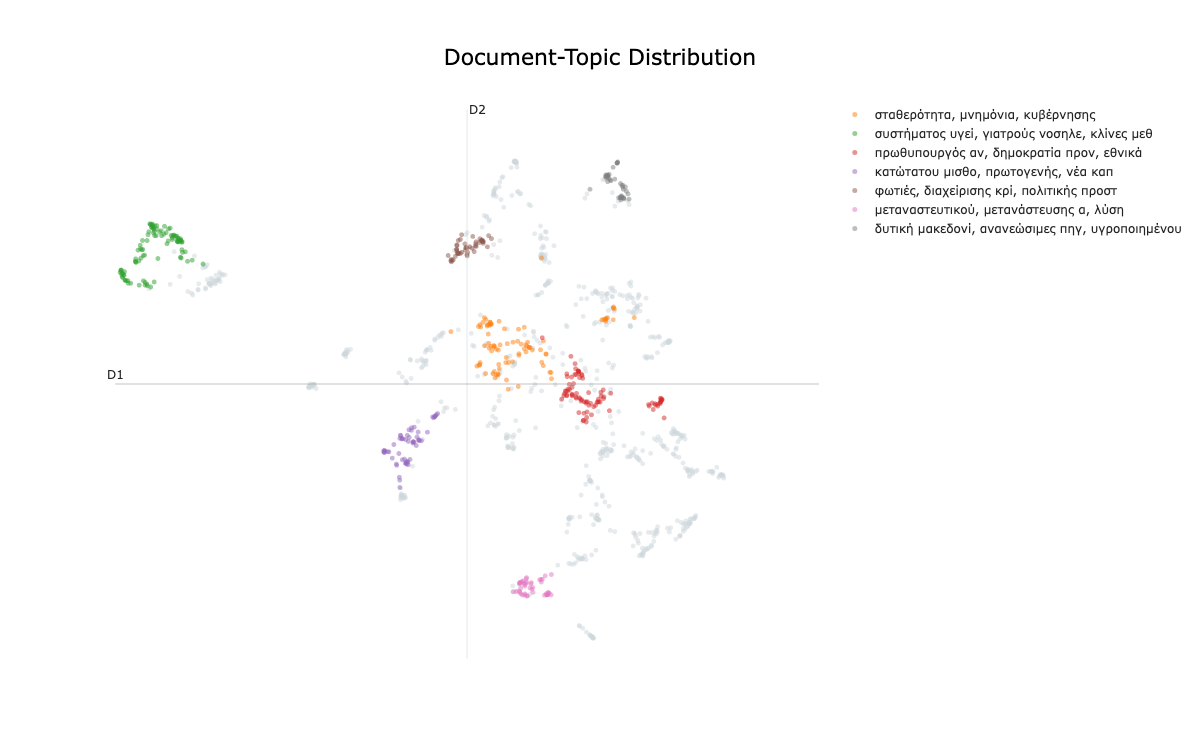
\includegraphics[width=1\columnwidth]{figs/document_topic_plot.png}
\label{fig:doc_topic_plot}
\end{figure}
\section{Evaluation and Discussion}
\label{sec:Discussion}

Going into this task, we were aware of the challenges when it comes to evaluating topic models - the results, however, are even more concerning than what we initially expected. As we see in Table \ref{tab:quant_metrics}, the quantitative evaluation of in our models seems to be especially confusing. We made the choice of tuning our models based on CV Coherence, which in retrospect appears to be far from the ideal coherence measure - raising concerns about whether our optimization achieved the best possible, and interpretable, results. However, this also seems to be the case with UMass. According to our empirical evaluation based on Table \ref{tab:best_model_topics}, BERTopic+ and ProdLDA produced the best topics. This is where the incoherence of coherence starts - with ProdLDA having the worst UMass and the best CV coherence scores, and BERTopic+ having a CV score that we would, unless we had seen the topics, discard immediately. On the other hand, Topic Diversity and Pairwise-Jaccard Similarity seem to be directly correlated with our empirical evaluation. 

Qualitative results are presented in Table \ref{tab:best_model_topics}, where the strictness of the ProdLDA preprocessing is apparent due to the absence of irrelevant words and the diversity of topics. On the other hand, BERTopic seems to suffer from poor topic representations. This is visible on Topic 4, with the words "que, de, en, la, el" being the prime representation words for that topic. BERTopic+ has eliminated such noise and was able to produce richer topics. On the analytical side, as expected, all of the algorithms produced topics related to economy, external policies, healthcare, infrastructure, democracy, COVID-19, immigration and other political cliches. For brevity reasons, not all topics are shown, with more niche topics being shadowed. Finally, Figure \ref{fig:doc_topic_plot} presents how the top topic clusters of BERTopic+ are distributed. They are clearly distinct with no overlap, something attributed to the optimized UMAP dimensionality reduction as well as the HDBSCAN clustering. It is safe to say that our top-performing models, in combination with our preliminary work, are able to achieve notable results.


\section{Conclusion and Future Work}
\label{sec:Conclusion}
This project started off as an analytical task, but quickly transitioned to a optimization and research project, as the fine-tuning and optimization of topic modeling algorithms proved to be far more exciting with a lot of depth to explore. We broke away from the defaultness of black-box pre-processing algorithms by constructing tailored pipelines and optimizing legacy algorithms to their best capabilities, allowing them to generate topics up to par with the state-of-the-art. Algorithms such as LSI, LDA, HDP and ProdLDA were put on the spot against BERTopic, which offers a variety of conveniences and is justifiably sitting at the SOTA throne for topic models. The ambiguity of quantitatively evaluating unsupervised topic models was a constant concern that led to a lot of second-guessing and the human factor was crucial to finding the best model.

Our work sets the baseline for unsupervised topic modeling in Hellenistic corpora, with a key takeaway being that English-based approaches such as spaCy and multilingual sentence transformers are outperformed by niche, yet well tailored, toolkits and models. The analysis was not groundbreaking - it was no surprise to anyone that Greece went over an economic crisis or that COVID-19 was a very hot topic - but the frozen-in-time model approach offered a retrospective view that while not as interesting, is certainly accurate and can prove useful in real-world scenarios.

Due to limitations in both time and project length, only the iceberg of our findings was presented. As an additional contribution to the field, all of our analysis is available in the project's open-source repository \citep{Rigatos;Giannakopoulos:24}. Further experimentation with an alternative input data granularity (sentences, paragraphs) and a more generous topic allowance could result in deeper insights with regards to understated events. Finally, additional approaches such as zero-shot, multi-modal and dynamic (over time) topic modeling make for interesting tasks to be tackled, especially in Greek.

% include your own bib file like this:
\bibliographystyle{plainnat}
\bibliography{bibliography}

\appendix
\appendix
\section{Architecture}
\label{sec:appA}

\subsection{Common Words Per Year}
In Table \ref{appA:words_per_year} we present a more exhaustive list of the most common words found per year:

\begin{longtable}[H]{>{\raggedright\arraybackslash}p{1cm} >{\raggedright\arraybackslash}p{6cm} >{\raggedright\arraybackslash}p{4cm}}
\caption{Most Common Words by Year} \\
\toprule
\textbf{Year} & \textbf{Common Words} & \textbf{Topic Description} \\
\midrule
\endfirsthead
\toprule
\textbf{Year} & \textbf{Common Words} & \textbf{Topic Description} \\
\midrule
\endhead
\bottomrule
\endfoot
2024 & \textgreek{πανεπιστήμιο, εταιρεία, εκλογή, σχετικά, αγρότης} & University, Elections, Farmers \\
2023 & \textgreek{φωτιά, τετραετία, τουρισμός, περιφέρεια, εκλογή} & Fire, Tourism, Elections \\
2022 & \textgreek{ενεργειακός, ψηφιακός, τουρισμός, πηγή, πόλεμος} & Energy, Digital, Tourism, War \\
2021 & \textgreek{εμβολιασμός, ψηφιακός, εμβολιάζω, υφυπουργός, γραμματέας} & Vaccines, Digital Campaigns \\
2020 & \textgreek{τουρισμός, νησί, νοσοκομείο, ψηφιακός, κορονοϊός} & Tourism, COVID-19 \\
2019 & \textgreek{βουλευτής, εκλογή, ψηφίζω, πλειοψηφία, κόμμα} & Elections \\
2018 & \textgreek{αναπτυξιακός, μνημόνιο, περιφέρεια, παραγωγικός, δημοσιονομικός} & Development, Memorandum \\
2017 & \textgreek{παραγωγικός, περιφέρεια, αναπτυξιακός, παραγωγή, σχεδιασμός} & Production, Regional Development \\
2016 & \textgreek{νησί, διαπραγμάτευση, δικαιοσύνη, κόμμα, αξιολόγηση} & Island Politics, Justice \\
2015 & \textgreek{κυπραίικος, βέβαιος, διαπραγμάτευση, βουλευτής, τράπεζα} & Cyprus Issue, Banking \\
2014 & \textgreek{ευρώ, οικονομικό, κρίση, σχέδιο, ανάκτηση} & Economic Crisis, Recovery Plan \\
2013 & \textgreek{πλεόνασμα, κόμμα, ανταγωνιστικότητα, πρωτογενής, ανεργία} & Surplus, Competitiveness, Unemployment \\
2012 & \textgreek{ανταγωνιστικότητα, ανταγωνισμός, competitiveness, αποκαθιστώ, διατηρώ} & Competitiveness, Market Dynamics \\
\bottomrule
\label{appA:words_per_year}
\end{longtable}

\section{Experimental Setup}
\label{sec:appB}
\subsection{Evaluation Metrics}
\begin{figure}[H]
\centering
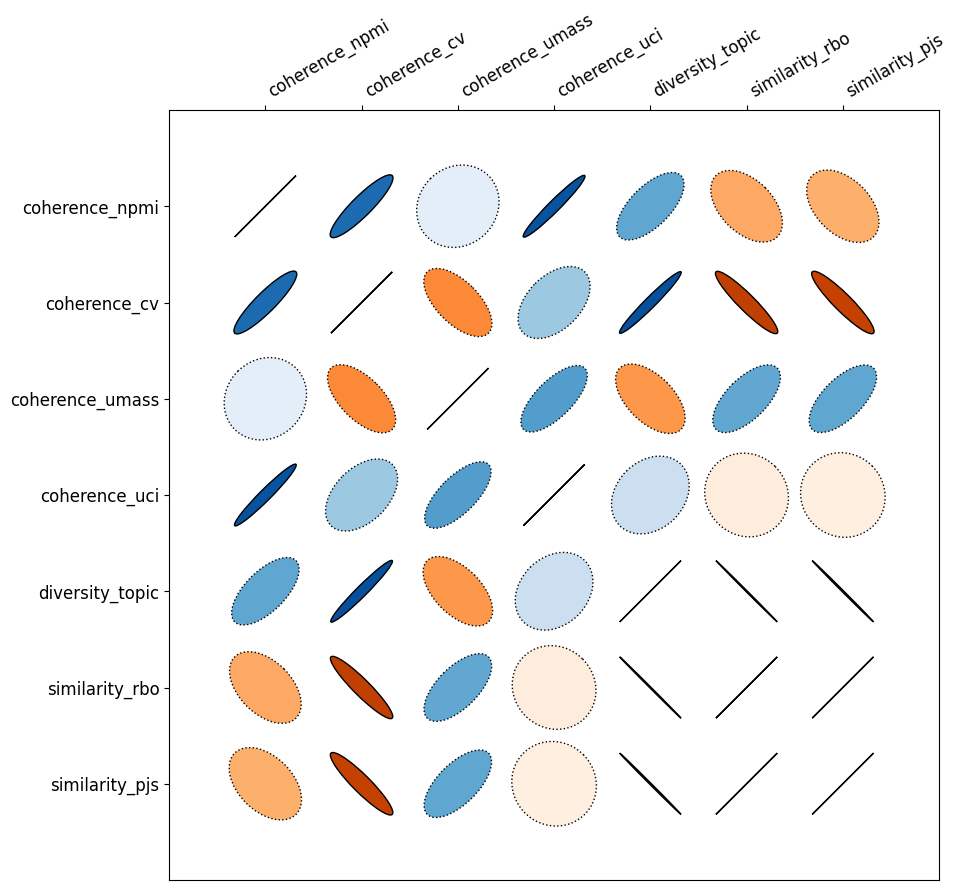
\includegraphics[width=1\columnwidth]{figs/metric_correlations.png}
\caption[Topic Modeling Metric Correlation Matrix]{Metric Correlation Matrix}
\label{appB:metric_correlations}
\end{figure}

\subsection{Hyperparameters}

Below we present the lists of hyperparameters for the NMF model:

\begin{table}[H]
\centering
\begin{tabular}{@{}lc@{}}
\toprule
Parameter           & Value   \\
\midrule
kappa               & 1.0     \\
minimum\_probability& 0.0543  \\
\bottomrule
\end{tabular}
\caption{NMF Hyperparameters}
\end{table}

\subsection{Sentence Transformers}
Document-level granularity models performed significantly better when it comes to the metrics, something we expected because of the constrained amount of topics. Without the topic limitation, sentence-level models produced thousands of topics - with BERTopic's automatic topic reduction not reducing them below four digits. This bottleneck renders their purpose useless and while it would certainly be an interesting topic (pun intended) to explore, it seems out of scope for this analysis.
\begin{table}[h]
    \centering
    \begin{tabular}{@{}lcc@{}}
        \toprule
        Model               & CV Coherence & Topic Diversity \\ 
        \midrule
        gr\_r\_xlm\_sentences       & 0.5019      & 0.9793          \\
        gr\_media\_sentences & \textbf{0.6041}      & \textbf{1.0000}       \\
        multilingual\_sentences & 0.5826  & 0.9724          \\
        gr\_r\_xlm\_docs            & 0.6826    & \textbf{0.7310}          \\
        gr\_media\_docs     &  0.6865    & 0.7241          \\
        multilingual\_docs   & \textbf{0.7024}     & 0.6087          \\
        \bottomrule
    \end{tabular}
    \caption{Model Evaluation on CV Coherence and Topic Diversity}
    \label{appB:st_eval}
\end{table}


\subsection{Topic Representations}
\label{sec:appendix_rep}
As previously mentioned, quantitative metrics aren't reliable measures of the quality of the topics. This becomes more apparent when changing the representation model. The default c-TF-IDF model, as seen in Table \ref{tab:coherence} yields better metrics, but different representations, as seen in Table \ref{tab:topics_compare}, make the topics much more human interpretable.


\begin{table}[h]
\centering
\begin{tabular}{lccc}
\toprule
 & CV Coherence  & UMass Coherence & Topic Diversity \\
\midrule
Default Representation Model & 0.646 & -0.518 & 0.935 \\
Custom Representation Model & 0.335 & -0.592 & 0.957 \\
\bottomrule
\end{tabular}
\caption{Topic Coherence Metrics}
\label{tab:coherence}
\end{table}

\begin{table}[H]
\centering
\begin{tabular}{ll}
\toprule
Default representation & Custom representation \\
\midrule
que, de, en, la, el & \textgreek{δημοκρατία, προνομιακός, μεταρρυθμίσεις} \\
\textgreek{ευρώ, μητσοτάκη, κύριε μητσοτάκη} & \textgreek{σταθερότητα, μνημόνια, κυβέρνηση} \\
\bottomrule
\end{tabular}
\caption{Comparison of Default and Custom Representations}
\label{tab:topics_compare}
\end{table}

\section{Experiments}

\subsection{Best Model Topic Representations}
\label{sec:appExpBest}

\begin{table}[H]
\caption{Top 8 most common topics for the best performing models (in English)}
{\footnotesize 
\begin{tabular}{|c|m{4cm}|m{4cm}|m{4cm}|}
\hline
\textbf{Topic} & \textbf{ProdLDA} & \textbf{BERTopic+} & \textbf{BERTopic} \\
\hline
1 & Obligated, clearance, entrance, minute, overcharge, mouth, enumerate, analyst, objectively & Government, solution, state, reforms, debt, you know, national & \textit{democracy, reforms}, euro, region, development, European, agreement \\
\hline
2 & Energy, presidency, directive, regulation, ultimate, ready, multi-year, adoption, migration, unemployment & Stability, memorandums, government, parliament, reforms, debt, Greek people & Tsipras, elections, Mitsotakis, SYRIZA, euro, Mr. Mitsotakis, ladies gentlemen \\
\hline
3 & Partner, negotiation, regulation, radical, administration, suffocating, institutional, eurozone, claiming, tax & Health system, doctors, nurses, beds, ICU, hospitals, health, Vasilis, vaccination, intensive care & Health, hospital, health system, hospitals, vaccination, national system, system \\
\hline
4 & Freedom, democratic, tolerance, against, racism, order, stereotypes, extremism, enemy, ethos & Prime Minister, Antonis, democracy, privileged, national, interests, simply, EAB, presidency & \textit{que, de, en, la, el}, Samaras, democracies \\
\hline
5 & Clearance, obligated, disastrous, mouth, entrance, writing, stock market, similar, apportion & Minimum wage, primary, new, CAP, minimum, livestock farmers, restaurant industry, businesses & Farmers, agricultural, products, agricultural, primary, sector, products, disability \\
\hline
6 & Hospital, personnel, doctor, care, primary, patient, cancer, governance, nurse, manager & Fires, crisis management, civil protection, EKAB, firefighting, civil protection, citizen, floods & Civil protection, protection, EKAB, civil protection, policy, firefighting, fires, police \\
\hline
7 & City, metro, museum, schedule, kilometer, Olympic, road, station, sports, regeneration & Immigration, asylum, solution, pact, migration, EU, Turkey, identification, flows & Flows, Frontex, refugees, Turkey, border, migration, borders \\
\hline
8 & Needs, add, table of appearances & Western Macedonia, renewable sources, liquefied, ELPE, FSRU, pipeline, ADMIE & Gas, energy, natural gas, natural gas, natural gas, natural \\
\hline
\end{tabular}}
\begin{tablenotes}
\small
\item \textit{Words in italics were found in the same language as presented here}
\end{tablenotes}
\label{appTab:english_topics}
\end{table}
% alternative, if using biber as backend
% \printbibliography

% It is not necessary to include any appendices, but if you do, add them at the very end of the document
%\input{appendices/appendices}

\end{document}
